\documentclass[tikz,border=10pt]{standalone}
\usepackage{tikz}
\usepackage{amsmath}
\usepackage{xcolor}
\usetikzlibrary{shapes,arrows,positioning,calc}

% Define colors
\definecolor{phase1}{RGB}{46, 125, 50}      % Foundation - Green
\definecolor{phase2}{RGB}{30, 136, 229}     % Growth - Blue  
\definecolor{phase3}{RGB}{255, 152, 0}      % Scale - Orange
\definecolor{phase4}{RGB}{156, 39, 176}     % Optimization - Purple
\definecolor{milestone}{RGB}{244, 67, 54}   % Milestones - Red
\definecolor{background}{RGB}{248, 249, 250}

\begin{document}
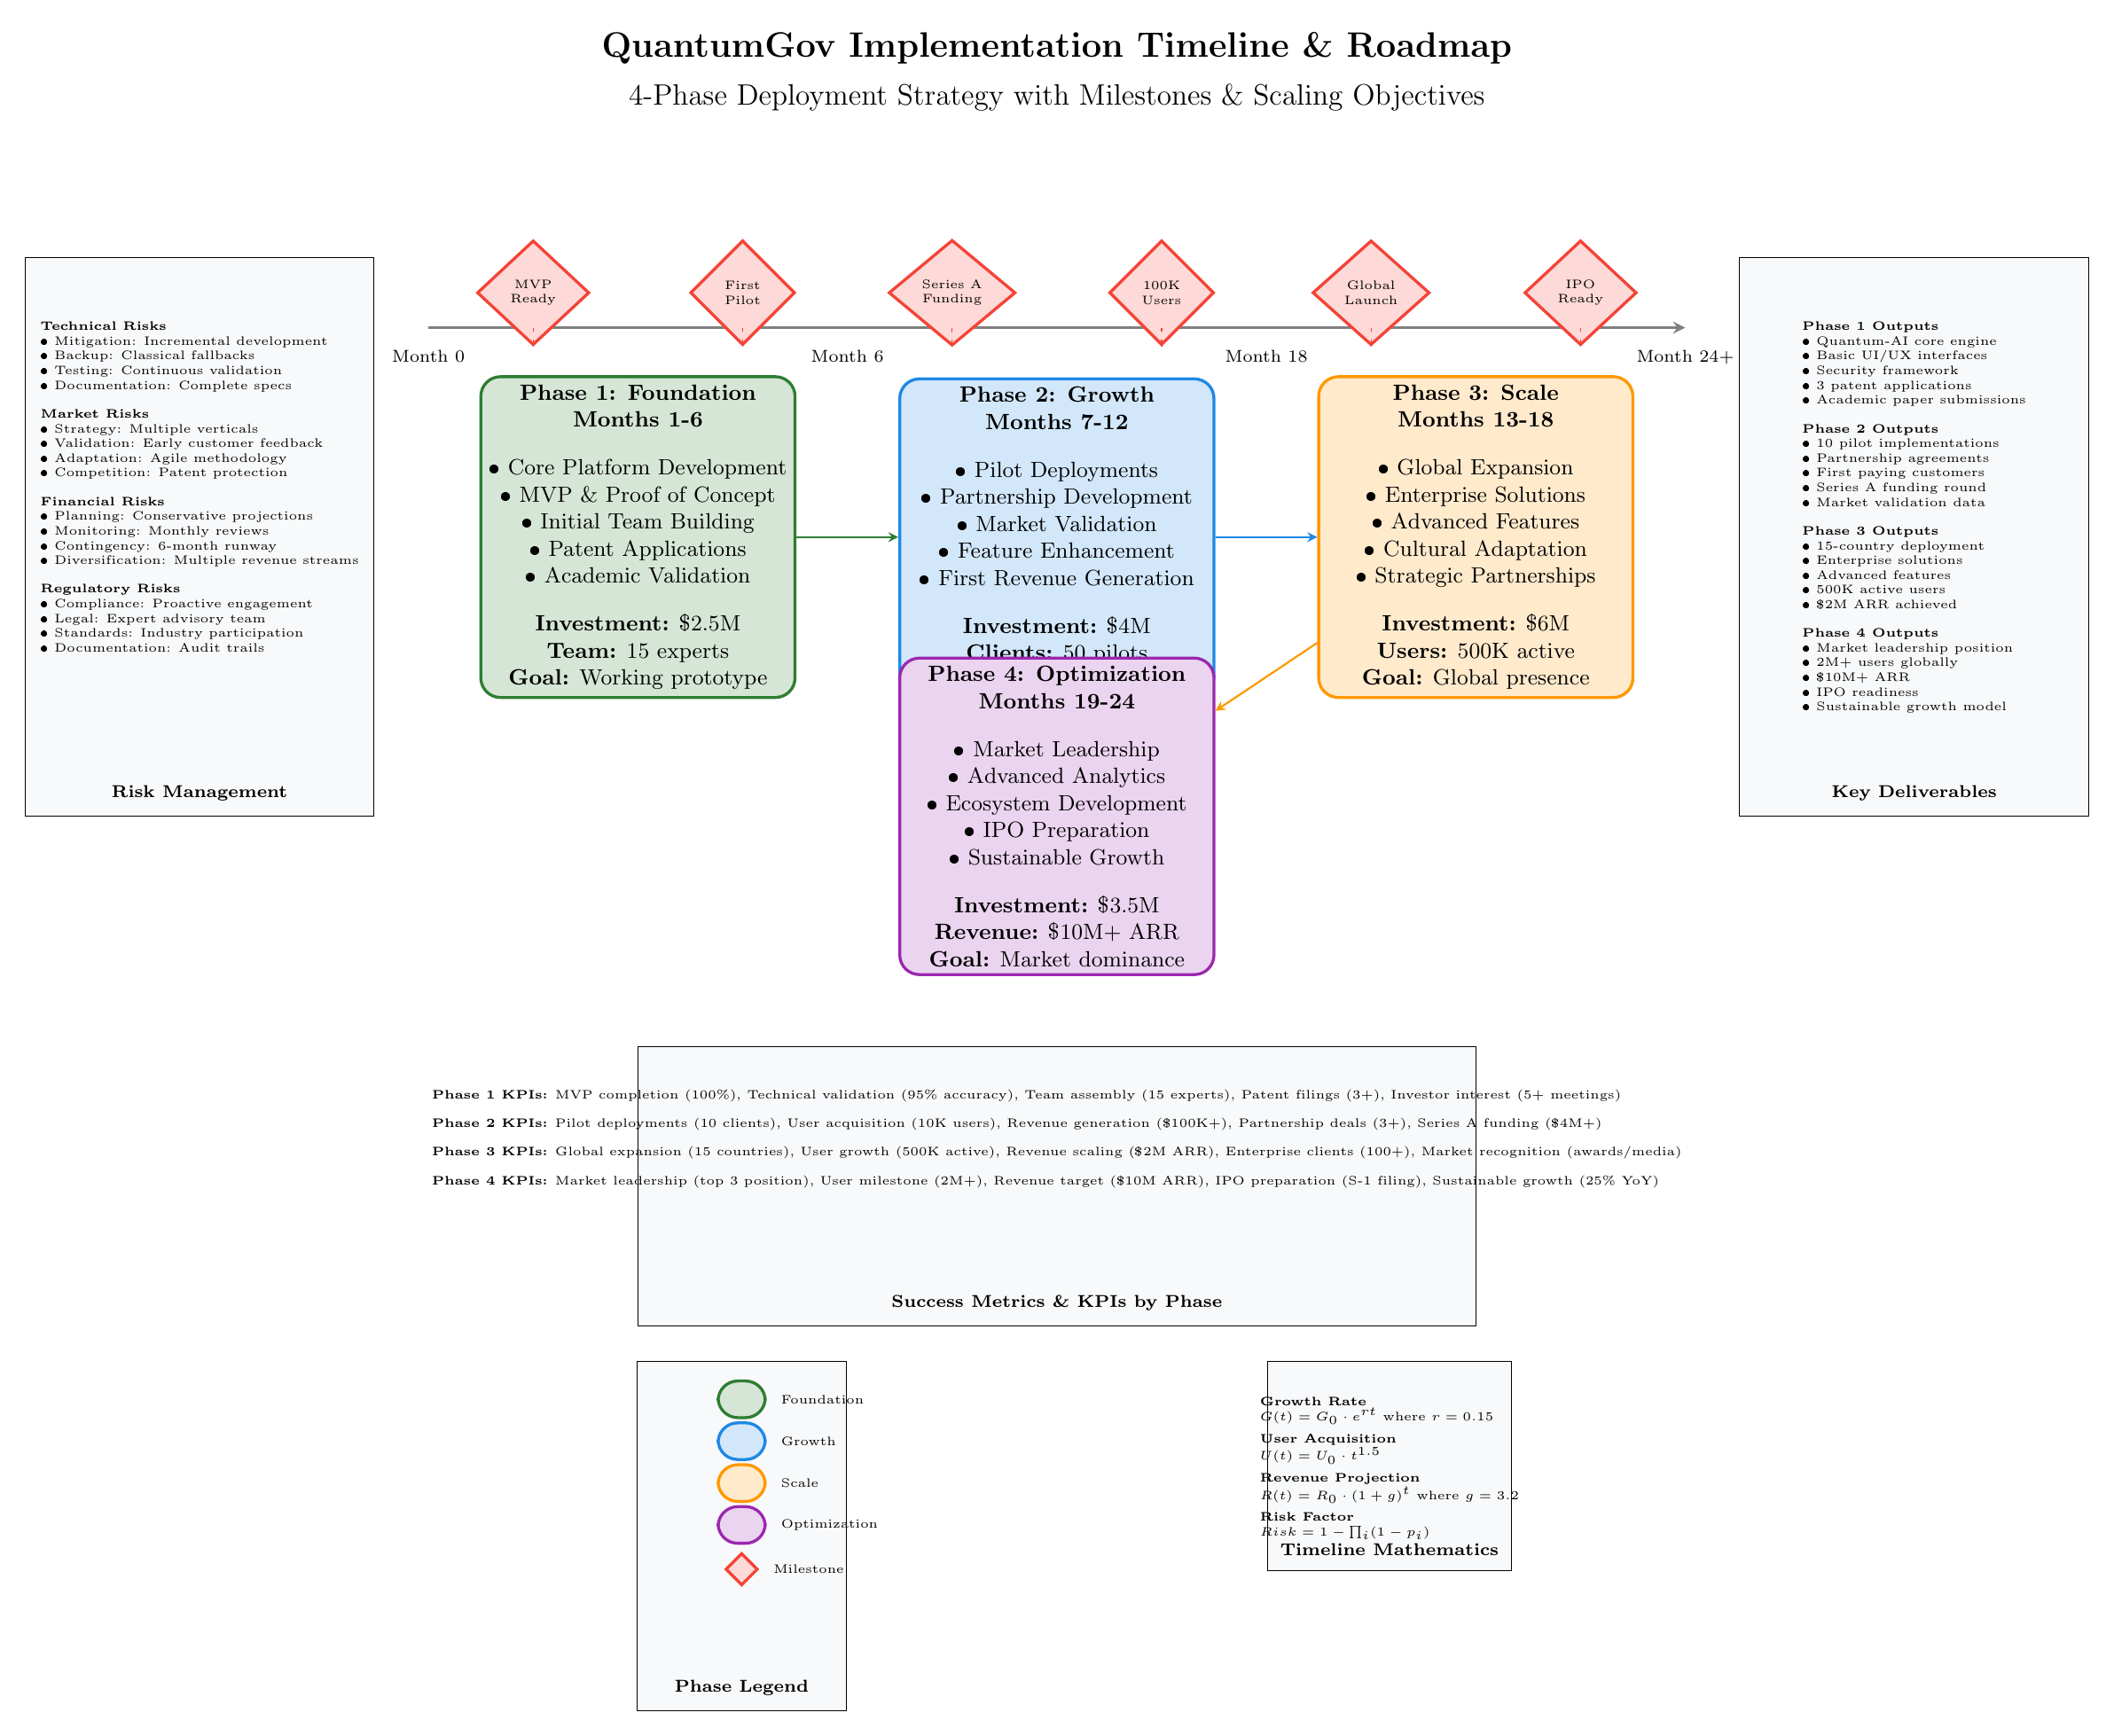
\begin{tikzpicture}[
    node distance=1cm,
    phase_box/.style={rectangle, rounded corners=8pt, draw, minimum height=3.5cm, minimum width=4.5cm, align=center, font=\small, very thick},
    milestone_node/.style={diamond, draw=milestone, fill=milestone!20, minimum size=1.5cm, align=center, font=\tiny, very thick, aspect=1.2},
    timeline_line/.style={->, very thick, >=stealth, color=gray},
    phase_arrow/.style={->, thick, >=stealth}
]

% Title
\node[align=center, font=\Large\bfseries] at (0, 16) {QuantumGov Implementation Timeline \& Roadmap};
\node[align=center, font=\large] at (0, 15.3) {4-Phase Deployment Strategy with Milestones \& Scaling Objectives};

% Timeline Base Line
\draw[timeline_line] (-9, 12) -- (9, 12);
\node[below=0.2cm of {(-9,12)}, font=\scriptsize] {Month 0};
\node[below=0.2cm of {(-3,12)}, font=\scriptsize] {Month 6};
\node[below=0.2cm of {(3,12)}, font=\scriptsize] {Month 18};
\node[below=0.2cm of {(9,12)}, font=\scriptsize] {Month 24+};

% Phase 1: Foundation (Months 1-6)
\node[phase_box, draw=phase1, fill=phase1!20] (phase1) at (-6, 9) {
    \textbf{Phase 1: Foundation}\\
    \textbf{Months 1-6}\\[0.3cm]
    • Core Platform Development\\
    • MVP \& Proof of Concept\\
    • Initial Team Building\\
    • Patent Applications\\
    • Academic Validation\\[0.3cm]
    \textbf{Investment:} \$2.5M\\
    \textbf{Team:} 15 experts\\
    \textbf{Goal:} Working prototype
};

% Phase 2: Growth (Months 7-12)  
\node[phase_box, draw=phase2, fill=phase2!20] (phase2) at (0, 9) {
    \textbf{Phase 2: Growth}\\
    \textbf{Months 7-12}\\[0.3cm]
    • Pilot Deployments\\
    • Partnership Development\\
    • Market Validation\\
    • Feature Enhancement\\
    • First Revenue Generation\\[0.3cm]
    \textbf{Investment:} \$4M\\
    \textbf{Clients:} 50 pilots\\
    \textbf{Goal:} Market traction
};

% Phase 3: Scale (Months 13-18)
\node[phase_box, draw=phase3, fill=phase3!20] (phase3) at (6, 9) {
    \textbf{Phase 3: Scale}\\
    \textbf{Months 13-18}\\[0.3cm]
    • Global Expansion\\
    • Enterprise Solutions\\
    • Advanced Features\\
    • Cultural Adaptation\\
    • Strategic Partnerships\\[0.3cm]
    \textbf{Investment:} \$6M\\
    \textbf{Users:} 500K active\\
    \textbf{Goal:} Global presence
};

% Phase 4: Optimization (Months 19-24)
\node[phase_box, draw=phase4, fill=phase4!20] (phase4) at (0, 5) {
    \textbf{Phase 4: Optimization}\\
    \textbf{Months 19-24}\\[0.3cm]
    • Market Leadership\\
    • Advanced Analytics\\
    • Ecosystem Development\\
    • IPO Preparation\\
    • Sustainable Growth\\[0.3cm]
    \textbf{Investment:} \$3.5M\\
    \textbf{Revenue:} \$10M+ ARR\\
    \textbf{Goal:} Market dominance
};

% Milestones
\node[milestone_node] (m1) at (-7.5, 12.5) {MVP\\Ready};
\node[milestone_node] (m2) at (-4.5, 12.5) {First\\Pilot};
\node[milestone_node] (m3) at (-1.5, 12.5) {Series A\\Funding};
\node[milestone_node] (m4) at (1.5, 12.5) {100K\\Users};
\node[milestone_node] (m5) at (4.5, 12.5) {Global\\Launch};
\node[milestone_node] (m6) at (7.5, 12.5) {IPO\\Ready};

% Phase Connections
\draw[phase_arrow, color=phase1] (phase1) -- (phase2);
\draw[phase_arrow, color=phase2] (phase2) -- (phase3);
\draw[phase_arrow, color=phase3] (phase3) -- (phase4);

% Milestone Connections to Timeline
\draw[dashed, color=milestone] (m1) -- (-7.5, 12);
\draw[dashed, color=milestone] (m2) -- (-4.5, 12);
\draw[dashed, color=milestone] (m3) -- (-1.5, 12);
\draw[dashed, color=milestone] (m4) -- (1.5, 12);
\draw[dashed, color=milestone] (m5) -- (4.5, 12);
\draw[dashed, color=milestone] (m6) -- (7.5, 12);

% Key Deliverables Panel
\node[draw, fill=background, minimum width=5cm, minimum height=8cm, right=1.5cm of phase3] (deliverables) {};
\node[above=0.1cm of deliverables.south, font=\scriptsize\bfseries, align=center] {Key Deliverables};
\node[below=0.8cm of deliverables.north, font=\tiny, align=left] {
    \textbf{Phase 1 Outputs}\\
    • Quantum-AI core engine\\
    • Basic UI/UX interfaces\\
    • Security framework\\
    • 3 patent applications\\
    • Academic paper submissions\\[0.2cm]
    \textbf{Phase 2 Outputs}\\
    • 10 pilot implementations\\
    • Partnership agreements\\
    • First paying customers\\
    • Series A funding round\\
    • Market validation data\\[0.2cm]
    \textbf{Phase 3 Outputs}\\
    • 15-country deployment\\
    • Enterprise solutions\\
    • Advanced features\\
    • 500K active users\\
    • \$2M ARR achieved\\[0.2cm]
    \textbf{Phase 4 Outputs}\\
    • Market leadership position\\
    • 2M+ users globally\\
    • \$10M+ ARR\\
    • IPO readiness\\
    • Sustainable growth model
};

% Risk Management Panel
\node[draw, fill=background, minimum width=5cm, minimum height=8cm, left=1.5cm of phase1] (risk_mgmt) {};
\node[above=0.1cm of risk_mgmt.south, font=\scriptsize\bfseries, align=center] {Risk Management};
\node[below=0.8cm of risk_mgmt.north, font=\tiny, align=left] {
    \textbf{Technical Risks}\\
    • Mitigation: Incremental development\\
    • Backup: Classical fallbacks\\
    • Testing: Continuous validation\\
    • Documentation: Complete specs\\[0.2cm]
    \textbf{Market Risks}\\
    • Strategy: Multiple verticals\\
    • Validation: Early customer feedback\\
    • Adaptation: Agile methodology\\
    • Competition: Patent protection\\[0.2cm]
    \textbf{Financial Risks}\\
    • Planning: Conservative projections\\
    • Monitoring: Monthly reviews\\
    • Contingency: 6-month runway\\
    • Diversification: Multiple revenue streams\\[0.2cm]
    \textbf{Regulatory Risks}\\
    • Compliance: Proactive engagement\\
    • Legal: Expert advisory team\\
    • Standards: Industry participation\\
    • Documentation: Audit trails
};

% Success Metrics Below
\node[draw, fill=background, minimum width=12cm, minimum height=4cm, below=1cm of phase4] (success_metrics) {};
\node[above=0.1cm of success_metrics.south, font=\scriptsize\bfseries, align=center] {Success Metrics \& KPIs by Phase};
\node[below=0.5cm of success_metrics.north, font=\tiny, align=left] {
    \textbf{Phase 1 KPIs:} MVP completion (100\%), Technical validation (95\% accuracy), Team assembly (15 experts), Patent filings (3+), Investor interest (5+ meetings)\\[0.2cm]
    \textbf{Phase 2 KPIs:} Pilot deployments (10 clients), User acquisition (10K users), Revenue generation (\$100K+), Partnership deals (3+), Series A funding (\$4M+)\\[0.2cm]
    \textbf{Phase 3 KPIs:} Global expansion (15 countries), User growth (500K active), Revenue scaling (\$2M ARR), Enterprise clients (100+), Market recognition (awards/media)\\[0.2cm]
    \textbf{Phase 4 KPIs:} Market leadership (top 3 position), User milestone (2M+), Revenue target (\$10M ARR), IPO preparation (S-1 filing), Sustainable growth (25\% YoY)
};

% Legend
\node[draw, fill=background, minimum width=3cm, minimum height=5cm, below left=0.5cm and -3cm of success_metrics] (legend) {};
\node[above=0.1cm of legend.south, font=\scriptsize\bfseries, align=center] {Phase Legend};
\node[phase_box, scale=0.15, draw=phase1, fill=phase1!20, above=4.2cm of legend.south] (leg_phase1) {};
\node[right=0.1cm of leg_phase1, font=\tiny] {Foundation};
\node[phase_box, scale=0.15, draw=phase2, fill=phase2!20, above=3.6cm of legend.south] (leg_phase2) {};
\node[right=0.1cm of leg_phase2, font=\tiny] {Growth};
\node[phase_box, scale=0.15, draw=phase3, fill=phase3!20, above=3cm of legend.south] (leg_phase3) {};
\node[right=0.1cm of leg_phase3, font=\tiny] {Scale};
\node[phase_box, scale=0.15, draw=phase4, fill=phase4!20, above=2.4cm of legend.south] (leg_phase4) {};
\node[right=0.1cm of leg_phase4, font=\tiny] {Optimization};
\node[milestone_node, scale=0.3, above=1.8cm of legend.south] (leg_milestone) {};
\node[right=0.1cm of leg_milestone, font=\tiny] {Milestone};

% Timeline Mathematics
\node[draw, fill=background, minimum width=3.5cm, minimum height=3cm, below right=0.5cm and -3cm of success_metrics] (timeline_math) {};
\node[above=0.1cm of timeline_math.south, font=\scriptsize\bfseries, align=center] {Timeline Mathematics};
\node[below=0.4cm of timeline_math.north, font=\tiny, align=left] {
    \textbf{Growth Rate}\\
    $G(t) = G_0 \cdot e^{rt}$ where $r = 0.15$\\[0.1cm]
    \textbf{User Acquisition}\\
    $U(t) = U_0 \cdot t^{1.5}$\\[0.1cm]
    \textbf{Revenue Projection}\\
    $R(t) = R_0 \cdot (1 + g)^t$ where $g = 3.2$\\[0.1cm]
    \textbf{Risk Factor}\\
    $Risk = 1 - \prod_i (1 - p_i)$
};

\end{tikzpicture}
\end{document}